
\documentclass[12pt,letterpaper]{report}
\usepackage[margin=1in]{geometry}
\usepackage{graphicx}
\usepackage{amsmath}
\usepackage[font=small,labelfont=bf]{caption}

\begin{document}

\title{E153 Laboratory Assignment \#1}
\author{Courtney Keeler and Stephen Pinto\\
Harvey Mudd College}
\date{September 30, 2013}
\maketitle

\begin{center}
List of Materials:
\begin{itemize}
	\item Tektronix 2212 Oscilloscope
	\item Hewlett Packard 33120A Function generator
	\item Pomona 4550B (10X probe)
	\item Multimeter
\end{itemize}
\end{center}

\section*{Section A: Analog Oscilloscope vs. Digital Storage Oscilloscope}
\subsection*{Procedure}
\begin{enumerate}
	\item Turn on the Hewlett Packard 33120A Function generator, set the out term to High Z and the amplitude to 1 $\text{V}_{\text{pp}}$
	\item Connect the of the function generator to the channel 1 input of the Tektronix 2212 Oscilloscope with a BNC cable
	\item Turn on digital storing on the oscilloscope (digital)
	\item Set the function generator frequency to 1 Hz and record the amplitude and frequency of the signal displayed by the oscilloscope
	\item Repeat the previous step with frequencies of 1kHz, 1MHz, and 10MHz
	\item Repeat the two previous steps with the oscilloscope's digital storing turned off (analog)
\end{enumerate}
\subsection*{Results}
\begin{table}[ht]
\caption{Presentation of Sin Waves} % title of Table
\centering 
    \begin{tabular}{| c | c | c |}
    \hline  
    Frequency & Analog & Digital \\
    \hline
    1 Hz & * & 283.1 m$\text{V}_{\text{pp}}$, 991.5 mHz \\
    1 kHz & 1.012 $\text{V}_{\text{pp}}$, 1.025 kHz & 1.003 $\text{V}_{\text{pp}}$, 1.002 kHz \\
    1 MHz & 1.003 $\text{V}_{\text{pp}}$, 1.003 MHz & 991.7 m$\text{V}_{\text{pp}}$, 1.00 MHz \\
    10 MHz & 976.2m$\text{V}_{\text{pp}}$, 10.06 MHz & ** \\
    \hline
    \end{tabular}
    \label{table:SinWave}
\end{table}
* Can see the sin wave moving across the screen but cannot capture samples and therefore cannot measure signal

** Can't be measured since time scale minimum is .4us/div while storing is on
\\[.1in]
Table \ref{table:SinWave} shows that the analog scope is favored for high frequency measurements, while the digital scope is favored for low frequency measurements. This is due to the fact that the analog oscilloscope cannot store past values, so at low frequencies, the oscilloscope displays a continuously moving signal. For a higher frequency signal, this is not an issue because the movement of the signal on the screen cannot be perceived by the human eye and appears static (and can therefore be measured). The digital oscilloscope can store past data points and therefore display a measurable signal at very low frequencies. However, the time required to perform an A/D conversion and store the value limits the upper frequency at which the digital oscilloscope can operate. While this setting stills displays data for a 10MHz signal, the user is unable to zoom far enough in on the screen to measure the frequency of the signal seen.

\section*{Section B.1: The 10X Scope Probe}
\subsection*{Procedure}
\begin{enumerate}
	\item Cut two pieces of wire and strip the both ends of each
	\item Insert one end of each wire in each slot of the capacitance measurement slot in the Multimeter
	\item Connect a BNC splitter to one end of a BNC/Coax cable
	\item Connect the positive lead of the splitter to the available end of the wire in the positive capacitance measurement terminal
	\item Repeat the above step for the negative lead and negative terminal
	\item Record the displayed capacitance
	\item Replace the BNC/Coax cable with the Pomona 4550B 10X probe (attaching probe tip to positive terminal and ground clip to negative terminal)
	\item Record the displayed capacitance
\end{enumerate}
\subsection*{Results}
\begin{center}
\begin{table}[ht]
\caption{Capacitance}
\centering
	\begin{tabular}{| c | c |}
	\hline
	
	BNC/Coax & 10X Probe \\
	\hline
	108 pF & 21 pF \\

	\hline
	\end{tabular}
\end{table}
\end{center}

\subsection*{Calculations}
The resistive and reactive loading are found by circuit analysis. For the BNC cable, the circuit is shown in Figure \ref{fig:bnc_circuit}.

\begin{figure}
	\centering
	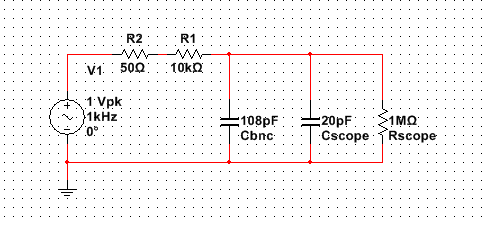
\includegraphics[width=\linewidth, keepaspectratio=true]{lab1_images/BNC_circuit.png} 
	\caption{Circuit model of a BNC cable connecting a function generator (with an additional 10k resistor in between) to an oscilloscope}
	\label{fig:bnc_circuit}
\end{figure}

We can see that the only resistive element is the 1M$\Omega$ resistor, so this resistance value becomes the resistive loading of the circuit. The circuit of the 10X probe is shown in Figure \ref{fig:probe_circuit}.

\begin{figure}
	\centering
	\includegraphics[width=\linewidth, keepaspectratio=true]{lab1_images/10x_circuit.png} 
	\caption{Circuit model of a 10x probe connecting a function generator (with an additional 10k resistor in between) to an oscilloscope}
	\label{fig:probe_circuit}
\end{figure}
 
Here we see that there are two resistive elements in series. The total resistive loading of this circuit becomes the sum of the two resistance values: 10M$\Omega$. These results are summarized in Table \ref{table:ResistiveLoading}.

\begin{center}
\begin{table}[ht]
\caption{Resistive Loading} % title of Table
\centering 
	\begin{tabular}{| c | c |}
	\hline
	
	BNC/Coax & 10X Probe \\
	\hline
	1 M$\Omega $ & 10 M$\Omega$ \\

	\hline
	\end{tabular}
	\label{table:ResistiveLoading}
\end{table}
\end{center}

To calculate the reactive loading of the BNC and 10X probe circuits, we analyze the capacitors only (if these circuits included inductors, they would be analyzed here too). For the BNC model, Figure \ref{fig:bnc_circuit} shows two capacitors in parallel. To find the total reactive loading, we add their values and find the impedance (Z) of the combined capacitance:
$$ \text{C}_{\text{total}} = 108 \text{pF} + 20 \text{pF} = 128 \text{pF} $$
$$ \text{Z} = \frac{1}{\text{j}\omega\text{C}_{\text{total}}} $$
The $\omega$ term refers to signal frequency, and we must evaluate for 100 Hz, 1kHz, and 1MHz. The results are summarized in Table \ref{table:ReactiveLoading}.

For the 10x probe model, Figure \ref{fig:probe_circuit} shows the only reactive elements are three capacitors - one in series with two in parallel. The total capacitance of these three capacitors is
$$ \text{C}_{\text{total}} = \frac{18 \text{pF} (53 \text{pF} + 20 \text{pF})}{18 \text{pF} + 53 \text{pF} + 20 \text{pF}} = 14 \text{pF} $$

 
\begin{center}
\begin{table}[ht]
\caption{Reactive Loading}
\centering
	\begin{tabular}{| c | c | c |}
	\hline	
	Frequency & BNC & 10X Probe \\
	\hline
	100 Hz & 12.4 M$\Omega$ & 110 M$\Omega$\\
	1000 Hz & 1.24 M$\Omega$ & 11.0 M$\Omega$\\
	1 MHz & 1.24 k$\Omega$ & 11.0 k$\Omega$\\	
	\hline
	\end{tabular}
	\label{table:ReactiveLoading}
\end{table}
\end{center}

\section*{Section B.2: The 10X Scope Probe}

For the 10X probe:
$$\text{C}_{\text{total}} = 14.4 \text{pF}$$
$$ \frac{1}{\omega \text{C}_{\text{total}}} = 10\text{M}\Omega$$
$$ \omega = 6.94 \text{kHz} $$

%
%Measure the capacitance of a BNC/Coax probe: .108nF (.011nF is the splitter alone, multimeter always shows .004 or .005 nF)
%
%Measure the input capacitance of the 10X probe (Pomona 4550B): 
%$C_{probe}$ = .013 nF
%$C_{equiv}$ = .021nF
%Sanity check: $C_{equiv}$ should work out to be $C_{probe}$ in series with $C_{BNC}$ (where $C_{BNC}$ = 0.053nF). 
%
%Nevermind, we ignore the capacitance due to the length of cable attached to the 10X probe.
%
% Experimental corner frequency for the BNC cable: 135 kHz (this is the frequency where the amplitude is .707)
% Multisim: 122.7 kHz difference: BNC splitter introduces another capacitor, multisim model doesn't include that or the resistance from the cables
% we measure the BNC splitter capacitance to verify: 12pF 
% Square wave: back to 1Vpp (909 mV). 10x corner: 164.2 mV, turned a square wave into a triangle wave
% Triangle: 678 mV (frequency limited (100kHz), can't scope it at corner frequency)
%
% Experimental corner frequency for the 10X probe:  (starting at 100mV) 1.15MHz
% Multisim: difference:
% square wave: 91.67 mV. 10x corner: 16.42 mV
% triangle wave: frequency limited
%

\end{document}